\documentclass[t]{beamer}
\usetheme{hkl}

\title{Research projects}
	\author{François Briatte \& Ivaylo Petev}
	\date{Week~\#12}

\begin{document}
    
    \frame[plain]{
        \titlepage\\[7em]
        \tableofcontents[hideallsubsections]
        }
    
		%
		%

		% 1 register
		% 2 form team
		% 3 choose data
		% 4 choose variables
		% 5 draft 1
		% 6 associations
		% 7 correlations
		% 8 simple ols
		% 9 draft 2
		% 10 multiple regression
		% 11 logistic regression
		% 12 diagnostics


	% ------ WEEK 1 -----------------------------------------------------------
	%
    \section*{Week 1}

	%
	\begin{frame}[c]{Week~1}
		
		\begin{block}{Readings}

			\begin{itemize}
				\item Course syllabus
				\item Stata Guide, Sec.~1--4
			\end{itemize}

		\end{block}

		\begin{block}{Video tutorials}
			
			\begin{itemize}
				\item ``\href{http://youtu.be/Uq0IS4dRtEQ}{Introducing the software}''
				
				\item ``\href{http://youtu.be/AlEmUqMBx4A}{Using do-files}''
			\end{itemize}
		
		\end{block}

	\end{frame}

	%
	\begin{frame}[c]{Week~1}

		\begin{exampleblock}{Practice}

			\begin{itemize}
				\item Explore the \texttt{SRQM} folder
				\item Replicate \texttt{week1.do}
			\end{itemize}
		
		\end{exampleblock}
		
		\begin{block}{How to replicate}
			
			\begin{itemize}
				\item Open the do-file: \texttt{doedit replication/week1}
				\item Read comments and run commands sequentially
			\end{itemize}

		\end{block}

		\begin{alertblock}{Important}
			Make sure the \texttt{SRQM} folder is the working directory.
		\end{alertblock}

	\end{frame}

	%
	\begin{frame}[c]{Week~1}

		\begin{alertblock}{Project}

			\begin{enumerate}
				\item Form a pair
				\item Choose a broad topic
				\begin{itemize}
					\item survey data: individuals, socioeconomic profiles, social and political attitudes…
					\item country-level data: nation-states, political institutions, macroeconomy, …
				\end{itemize}
				\item Register your group
			\end{enumerate}

		\end{alertblock}

		\vfill
		Project registration page: \url{http://goo.gl/brYmB}
		\vfill
						
	\end{frame}


	% ------ WEEK 2 -----------------------------------------------------------
	%
    \subsection*{Week 2}
	\begin{frame}[c]{Week~2: Explore the course datasets}
		
		\begin{block}{Learn a first set of commands}

			cd and ls
			d, lookfor

		\end{block}

		\begin{block}{Select a set of variables}

			Choose variables with low numbers of \red{missing values}.

		\end{block}

		\begin{alertblock}{Write up the dataset description}

			In one paragraph, describe the \red{sample design} and cite the \red{full data source} in a footnote.

		\end{alertblock}
				
	\end{frame}

	%
	\subsection*{Example of dataset description}
	\begin{frame}[c]{Example of dataset description}
		
		\begin{quote}
			 The General Social Survey (GSS) is an omnibus survey of the general US population. It covers years 1972--2004. Since it became biennial in 1994, it has asked about 1,000 questionnaire items to around 3,000 respondents per year through face to face interviews with a response rate of approximately 70\%. The sample design uses information from the U.S. Census to apply three stages of stratification to a hundred primary sampling units.\footnote{Smith, T. W. \emph{et al.} 2011. \emph{\href{http://publicdata.norc.org/GSS/DOCUMENTS/BOOK/GSS_Codebook_intro.pdf}{General Social Surveys, 1972-2010}} (codebook).\\[1em]}			
		\end{quote}
		
		\hfill Adapted from \href{http://www.unc.edu/~skolenik/talks/LinearRegressionPlus.pdf}{Stan Kolenikov, 2005}.

	\end{frame}
	
	%
	\begin{frame}[c]{Stata video tutorials}
    
        \href{https://www.youtube.com/watch?v=AlEmUqMBx4A&feature=plcp}{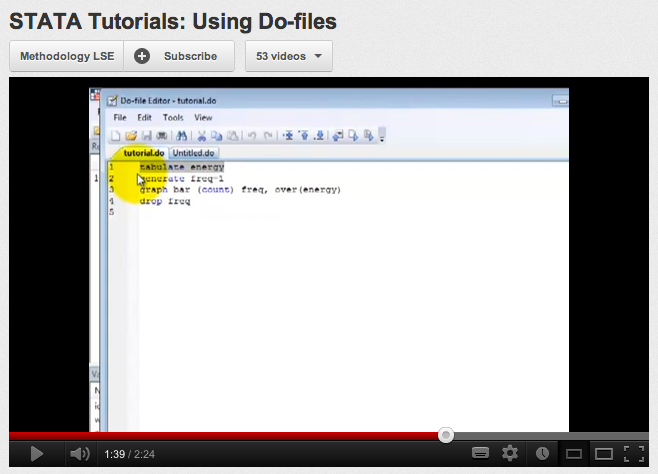
\includegraphics[width=.475\textwidth]{lse-tutorials-1}}%
		\hfill%
		\href{https://www.youtube.com/watch?v=0C_Hlh_jNq8&feature=plcp}{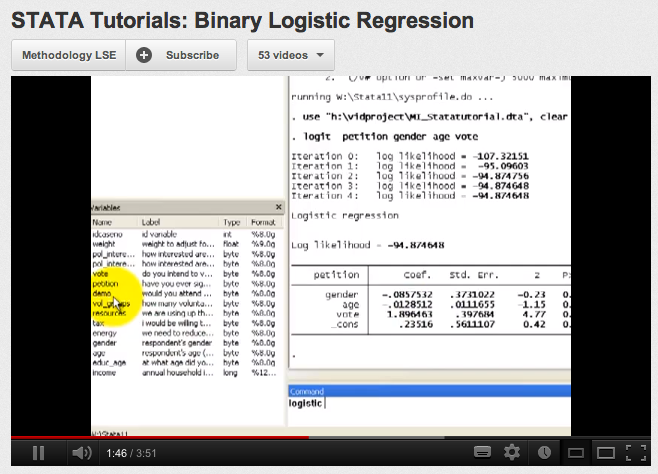
\includegraphics[width=.475\textwidth]{lse-tutorials-2}}% CHANGE THAT ONE
		%
		\vfill%
		%
		Source: \href{https://www.youtube.com/user/MethodologyLSE/videos?query=stata}{LSE Methodology Institute}, 2012.

    \end{frame}


	% ------ WEEK 3 -----------------------------------------------------------
	%
    \subsection*{Week 3}

	%
	\begin{frame}[c]{Week~3: Select a dataset}
		
		\begin{block}{Select a level of observation}

			Choose a \red{survey} (ESS, GSS, WVS) or \red{country-level} (QOG) dataset.

		\end{block}

		\begin{block}{Select a set of variables}

			Choose variables with low numbers of \red{missing values}.

		\end{block}

		\begin{alertblock}{Write up the variable descriptions}

			In two paragraphs, describe (1) the \red{dependent variable} and its distribution, and (2) the \red{independent variables} used as DV predictors.

		\end{alertblock}
				
	\end{frame}

	\subsection*{Example of variable descriptions}
	\begin{frame}[c]{Example of variable descriptions}
		
		\begin{quote}
			
		\end{quote}

	\end{frame}


	% ------ WEEK 4 -----------------------------------------------------------
	%
    \section*{Week 4}

	%
	\begin{frame}[c]{Week~4: Select variables}
		
		\begin{block}{Select one dependent variable (DV)}

			The DV must be \red{continuous} to a reasonable extent: do not select a variable with less than five dimensions or with high skewness.

		\end{block}

		\begin{block}{Select 6--12 independent variables (IVs)}

			Include \red{covariates} and socio-demographic and economic \red{controls} like age, sex, education, income, city size, etc.

		\end{block}

		\begin{alertblock}{Write up clear hypotheses}

			Justify your selection by briefly explaining how you expect each IV to influence the DV. \red{Read example papers}.

		\end{alertblock}
				
	\end{frame}


	% ------ WEEK 5 -----------------------------------------------------------
	%
    \section*{Week 5}

	%
	\section{Draft No. 1}

    \begin{frame}[t]{Week~5: \red{Draft No.~1}}
    
	    \begin{columns}[T]
	    \column{.3\textwidth}
	    \textbf{Univariate\\statistics}
    
	    \vspace{.55em}
	    \begin{itemize}
	        \item Introduction
	        \item Dataset
	        \item Variables
	    \end{itemize}

	    Assignment No. 1
    
	    $$
	    \left.
	        \begin{array}{rrr}
	            corrected \\
	            revised\\
	            appended
	        \end{array}
	    \right \}
	    $$
    
	    \column{.3\textwidth}
	    \textbf{Bivariate\\statistics}
    
	    \begin{itemize}
	        \item Associations
	        \item Correlations
	        \item Simple OLS
	    \end{itemize}
	    \red{Assignment No. 2}\\[.5em]
    
	    \fbox{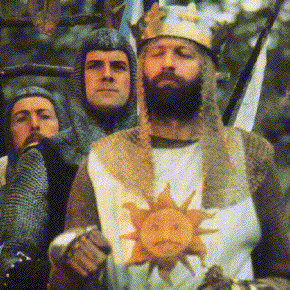
\includegraphics[width=.75\textwidth]{holy-grail2.jpg}}
    
	    \column{.3\textwidth}
	    \textbf{Statistical\\modelling}
    
	    \begin{itemize}
	        \item Regressions
	        \item Diagnostics
	        \item Conclusion
	    \end{itemize}
	    Final paper\\[.5em]
	    \fbox{
\includegraphics[width=.75\textwidth]{holy-grail.jpg}}
	    \end{columns}
    
    \end{frame}


	% ----------- * * * STAB --------------------------------------------------
	%
	\subsection{stab}

	\begin{frame}[t,fragile]{The \texttt{stab} command}

		\begin{block}{Syntax: \texttt{stab using Briatte\_Petev\_1, replace...}}

	        \begin{itemize}
	            \item \texttt{sum()} summarizes continuous variables
	            \item \texttt{fre()} summarizes categorical variables
	            \item \texttt{by()} creates multiple tables for comparison
	        \end{itemize}

			Add the \texttt{corr} option to also export a correlation matrix.

	    \end{block}

		\begin{exampleblock}{\texttt{use datasets/nhis2009, clear}}%
			\vspace{-1em}

	        \begin{verbatim}
stab using Briatte_Petev_1, replace ///
    sum(age weight height) corr ///
    fre(sex uninsured health) ///
    by(regionbr)\end{verbatim}

	    \end{exampleblock}

	\end{frame}

	\begin{frame}[c]{Stata video tutorials}

        \href{https://www.youtube.com/watch?v=AlEmUqMBx4A&feature=plcp}{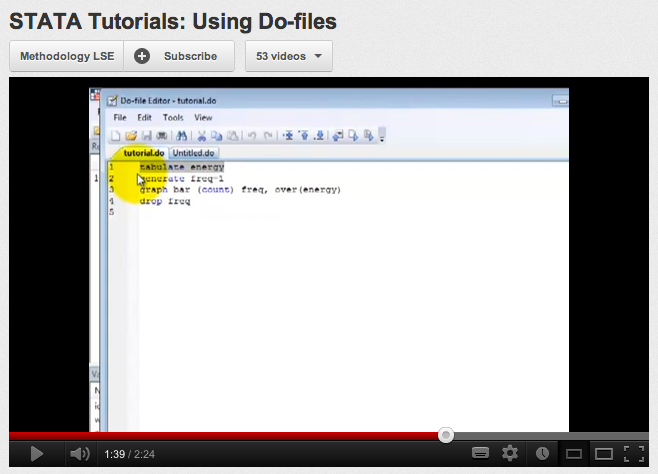
\includegraphics[width=.475\textwidth]{lse-tutorials-1}}%
		\hfill%
		\href{https://www.youtube.com/watch?v=0C_Hlh_jNq8&feature=plcp}{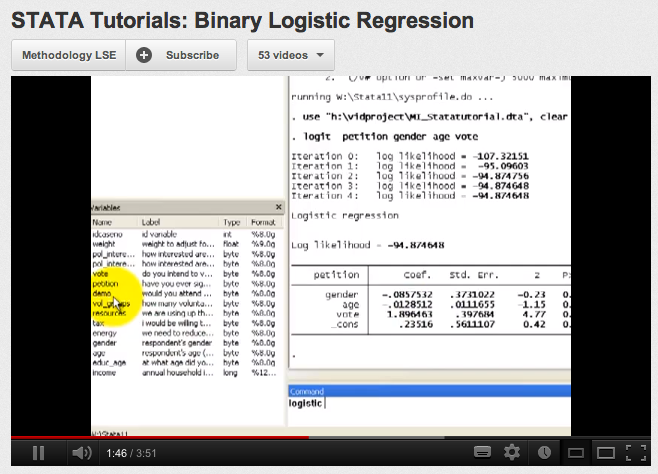
\includegraphics[width=.475\textwidth]{lse-tutorials-2}}%
		%
		\vfill%
		%
		Source: \href{https://www.youtube.com/user/MethodologyLSE/videos?query=stata}{LSE Methodology Institute}, 2012.

    \end{frame}


	% ------- WEEK 6 ----------------------------------------------------------
	%
    \section*{Week 6}


	% ------- WEEK 7 ----------------------------------------------------------
	%
    \section*{Week 7}


	% ------- WEEK 8 ----------------------------------------------------------
	%
    \section*{Week 8}


	% ------- WEEK 9 ----------------------------------------------------------
	%
	\section*{Week 9}

	%
	\section{Draft No. 2}
    
    \begin{frame}[t]{Week~9: \red{Draft No.~2}}
    
	    \begin{columns}[T]
	    \column{.3\textwidth}
	    \textbf{Univariate\\statistics}
    
	    \vspace{.55em}
	    \begin{itemize}
	        \item Introduction
	        \item Dataset
	        \item Variables
	    \end{itemize}

	    Assignment No. 1
    
	    $$
	    \left.
	        \begin{array}{rrr}
	            corrected \\
	            revised\\
	            appended
	        \end{array}
	    \right \}
	    $$
    
	    \column{.3\textwidth}
	    \textbf{Bivariate\\statistics}
    
	    \begin{itemize}
	        \item Associations
	        \item Correlations
	        \item Simple OLS
	    \end{itemize}
	    \red{Assignment No. 2}\\[.5em]
    
	    \fbox{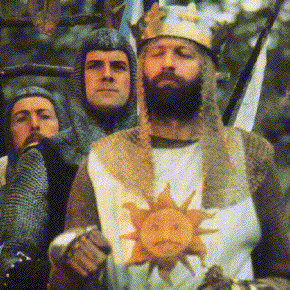
\includegraphics[width=.75\textwidth]{holy-grail2.jpg}}
    
	    \column{.3\textwidth}
	    \textbf{Statistical\\modelling}
    
	    \begin{itemize}
	        \item Regressions
	        \item Diagnostics
	        \item Conclusion
	    \end{itemize}
	    Final paper\\[.5em]
	    \fbox{
\includegraphics[width=.75\textwidth]{holy-grail.jpg}}
	    \end{columns}
    
    \end{frame}


	% ------- WEEK 9 ----------------------------------------------------------
	%
    \section*{Week 9}


	% ------- WEEK 10 ---------------------------------------------------------
	%
    \section*{Week 10}


	% ------- WEEK 11 ---------------------------------------------------------
	%
    \section*{Week 11}


	% ------- WEEK 12 ---------------------------------------------------------
	%
	\section*{Week 12}

	%
	%
	%	
	\section{Structure}
	
	\begin{frame}[t]{Structure}

	Use the IMRAD standard formatting:
		\begin{enumerate}
			\item \textbf{Introduction} to your \red{research design} (topic, theory, hypotheses).

			\item \textbf{Methods} made of \red{dataset} and \red{variable} descriptions.
			
			\item \textbf{Results} of bivariate \red{tests} and \red{regression} analysis.

			\item \textbf{Discussion}, where you provide an \red{appraisal} of your original theory.
		\end{enumerate}

	The final paper includes, approximately:

	\begin{itemize}
		\item \textbf{10--12 pages} all inclusive, with footnote references.
		
		\item \textbf{1--3 figures} of visually informative plots.
		
		\item \textbf{3--4 tables} to describe variables and cover results.
	\end{itemize}
	
	Precise instructions are all over the Stata Guide.
	
	Examples are everywhere in the course do-files.

	\end{frame}
		
	\subsection{Introduction}
	
	\begin{frame}[t]{Introduction (max. 1 page)}

		\begin{itemize}
			\item \textbf{Research question}: \\
			\begin{quote}``The aim of this study is to establish whether, in the United States, \textbf{obesity} \red{[dependent variable]} is determined by the \textbf{level of education} \red{[main independent variable]}, and how this effect varies across \textbf{race groups} \red{[comparison of groups]}.''\end{quote}
			
			% under which circumstances and to what extent
			
			\item \textbf{Context}: \\
			\begin{quote}``Obesity has \textbf{increased dramatically} since the 1980s \red{[magnitude]} and contributes to \textbf{social distinction} \red{[theory]}.''\end{quote}
			
			\item \textbf{Hypotheses}: \\
			\begin{quote}
				$\mathrm{H_1}$: ``All other things kept equal, \red{higher levels of education} are associated with \red{lower levels of obesity}.\\
				
				$\mathrm{H_2}$: The effect of education on obesity is \red{highest for African Americans} and weakest for \red{Asian Americans}.''\end{quote}
		\end{itemize}
		
	\end{frame}
	
	\subsection{Methods}

	\begin{frame}[t]{Methods (max. 2 pages)}

		\begin{itemize}
			\item \textbf{Dataset}: \\
			\begin{quote}``The  National Health Interview Survey \red{[cite source]} contains a measure of Body Mass Index for the American population \red{[cite the unit of analysis, sampling method and total number of observations for the dependent variable, as well as transformations or recoding]}.''\end{quote}

			\item \textbf{Variables}: \\
			\begin{quote}``The dependent variable is a continuous variable, which is constructed from \red{[cite the measurement method from the codebook]}. Its distribution is approximately normal over the sample \red{[describe normality]}. The variable is summarised, along with independent variables, in Table 1 \red{[include summary statistics and brief descriptions]}.''\end{quote}
		\end{itemize}

	\end{frame}

	\subsection{Results}
	
	\begin{frame}[t]{Results (max. 5 pages)}

		\begin{itemize}
			\item \textbf{Association}: \\
			
			\begin{quote}``We find a statistically strong association between obesity and education \red{[describe results through text with probability levels in brackets; reproduce the correlation matrix]}. The effect holds across ethnic groups \red{[show independent variables as controls in crosstabulations or graphs only when they are pertinent to your general argument]}.''
			\end{quote}

			\item \textbf{Regression}: \\
			\begin{quote}``The model for each ethnic group is reproduced in Table 3 \red{[include the regression output as a single table, with one column for each model]}. It establishes that education is a strong predictor of obesity, along with covariates such as age, and after controlling for income \red{[interpret R-squared and all coefficients: statistical significance, direction, magnitude]}.''\end{quote}
		\end{itemize}

	\end{frame}

	\subsection{Discussion}
	
	\begin{frame}[t]{Discussion (max. 2 pages)}

		The results will indicate \red{strong, moderate or weak effects} that either \red{confirm or reject} your background assumptions.
		
		\begin{itemize}
			\item Interpret \textbf{confirmatory results}: \\
			\begin{quote}``Our analysis provides clear evidence in support of the argument \red{[expressed in one of your hypotheses]} that… This corroborates the view that… \red{[support, reject or amend the theoretical priors on which your research design relies]}.''\end{quote}

			\item Also cover \textbf{negative results}: \\
			\begin{quote}``Our analysis provides no clear evidence in support of the argument \red{[expressed in another hypothesis]} that… This result challenges our intuition that…''\end{quote}

			Statistical insignificance can be attributed to sample size, measurement issues, or to a theory that might need revision.			
		\end{itemize}

	\end{frame}
	
	%
	%
	%
	\section{Inclusions}

	\begin{frame}[t]{Inclusions}
		\begin{columns}[T]
			\column{.5\textwidth}
			Some stuff \red{necessarily} goes into your paper to make your point and support the burden of proof.\vspace{1em}
			
			But it is just as important to realize that some stuff does \red{not} go into your paper.\vspace{1em}
			
			The manuscript on the right is from Hunter S. Thompson's \textit{Fear and Loathing in Las Vegas} (1971).
			\column{.4\textwidth}
			\href{http://www.theparisreview.org/interviews/619/the-art-of-journalism-no-1-hunter-s-thompson}{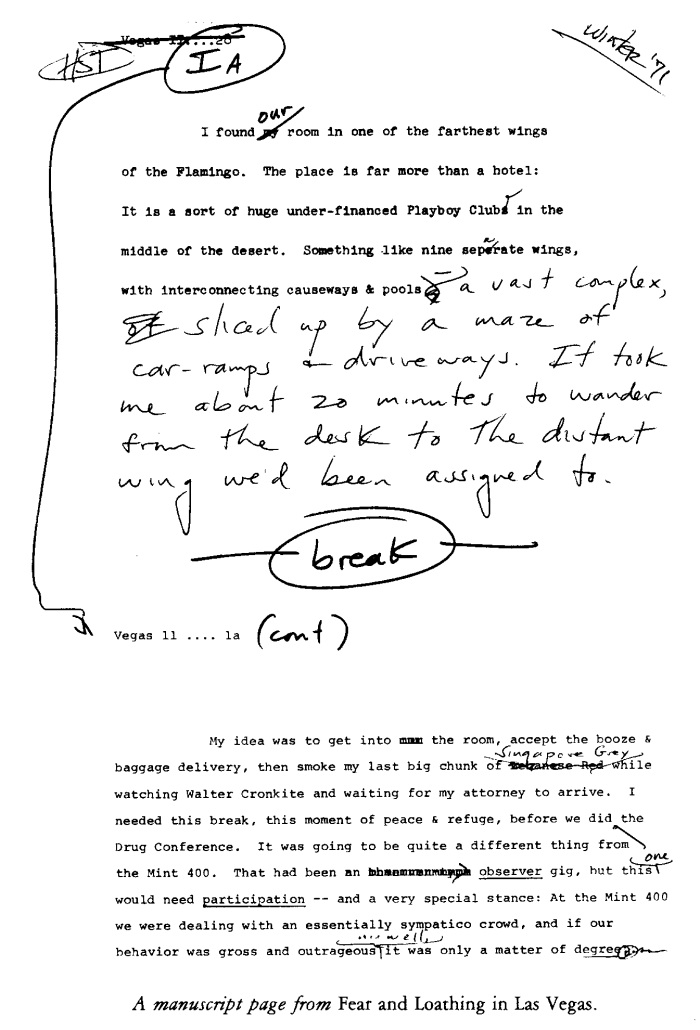
\includegraphics[height=.6\paperheight]{thompson.jpg}}
		\end{columns}
	\end{frame}
	
	\subsection{What to include}
	
	\begin{frame}[t]{What to include}

		\begin{itemize}

			\item \textbf{Sources} for all cited items:\\
				\begin{quote}``1. \red{Author(s)}, Dataset Name, \red{Year of Release} \textless\red{URL}\textgreater.''\end{quote}

			\item \textbf{Captions} for (numbered) tables and figures: \\
			\begin{quote}
			``\red{Fig. 2.} Dot graph showing the average level of subjective happiness by geographical region.''
			\end{quote}

			\item \textbf{Probability levels}: \\
			\begin{quote}``Given the strong correlation between happiness and wealth (\red{$r = 0.79, p < 0.01$}) we were not surprised to observe our dummy for Western states return a significant increase in happiness of \red{3.4 percentage points} at \red{$p < 0.05$} (\red{Table 4}).''\end{quote}

			\item \textbf{\red{Interpretation.}}

		\end{itemize}

	\end{frame}
	
	\subsection{Systematic interpretation}

	\begin{frame}[t]{Systematic \red{interpretation}}
		\begin{columns}[T]
			\column{.4\textwidth}
			If you forget to interpret your output, you will be thrown into the gaping mouth of the sarlaac that inhabits the Great Pit of Carkoon on planet Tatooine ($p < 0.01$).\vspace{1em}
			
			And kittens will get hurt.
			\column{.4\textwidth}
			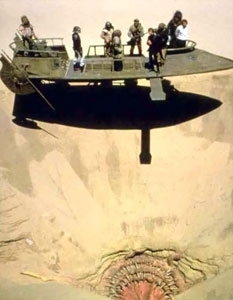
\includegraphics[height=.66\paperheight]{sarlaac.jpg}
		\end{columns}
	\end{frame}

	\subsection{Systematic references}

	\begin{frame}[t]{Systematic \red{references}}
		\begin{columns}[T]
			\column{.4\textwidth}
			If you forget to reference your sources, the hideous terror of Cthulhu will arise from the sunken city of R'lyeh to spread the abject curse of the Great Old Ones onto this world ($p < 0.01$).\vspace{1em}
		
			And kittens will get hurt. Again. Different ones.
			\column{.4\textwidth}
			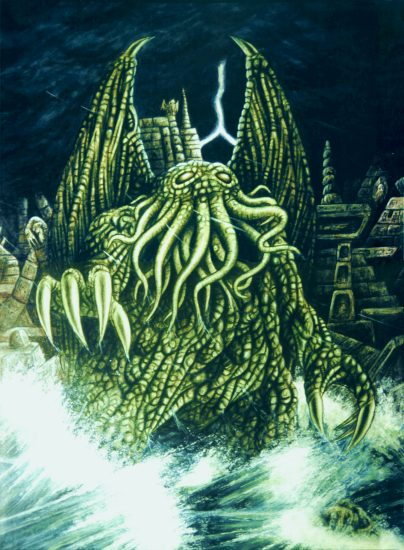
\includegraphics[height=.66\paperheight]{cthulhu.jpg}
		\end{columns}
	\end{frame}
	
	\subsection{What not to include}
	
	\begin{frame}[t]{What \textbf{\red{not}} to include}

		\begin{itemize}

			\item \textbf{Insignificant output}, even if you will comment on the negative findings in your Discussion.\\
			\begin{quote}
			``Look at that cute result with a \emph{p}-value of 0.697!''
			\end{quote}

			\item \textbf{Unexplained output}, in the form of (usually several) pasted extracts of Stata results with no solid interpretation.\\
			\begin{quote}
			``Have a look at Tables 4--12 and have fun reading them!''
			\end{quote}

			\item \textbf{Virtually every possible figure} created by your do-file, regardless of the actual information it might convey to the reader.\\
			\begin{quote}
			``Notice how good I am at producing scatterplots for \red{all} variables (see Fig. 7--77 and the 16-page Appendix H).''
			\end{quote}

			\item \textbf{\red{Causality.}}
		\end{itemize}

	\end{frame}
	
	\subsection{What to do with causality}
	
	\begin{frame}[t]{What to do with \red{causality}}
		
		The basic problem concerns your language: can you establish that $y$ is \red{``caused''} by $a + b_1x_1 + b_2x_2 + \epsilon$, given your regression results?\vspace{1em}

		A short answer is that:
		
		\begin{itemize}

			\item \textbf{Statistical equations provide the \red{conditional distribution}} of $y$ given $x_1$ and $x_2$, and its probability level. No more, no less.
			
			% 'species' = difference in nature (genus)
			% 'schismatic' because the notation is not commensurable
			% rift because they still both qualify nature
			\item \textbf{Causal and statistical information are \red{separate species}}. Reuniting them implies crossing a wide, schismatic rift.
		
		 	\item \textbf{Statistical inference basically requires a \red{background theory}} to meet the requirements of causal analysis in observational studies.
		\end{itemize}
		
		Further reading:
		
		\begin{itemize}
			\item \textbf{Judea Pearl}, ``\href{http://ftp.cs.ucla.edu/pub/stat_ser/r373-reprint.pdf}{Statistics and Causality}'' (2011).
		\end{itemize}
	\end{frame}

	\subsection{What the final package looks like}
	
	\begin{frame}[t]{The final package}

		\begin{itemize}
			\item \textbf{paper}\texttt{.pdf} using family names, e.g. \texttt{Briatte\_Petev.pdf}
			\item \textbf{do-file}\texttt{.do} using family names, e.g. \texttt{Briatte\_Petev.do}
			\item \textbf{dataset}\texttt{.dta} using acronym and year, e.g. \texttt{wdi2010.dta}\\[.5em] (only if you are using a dataset from outside the course)
		\end{itemize}
				
		The substantive qualities of your work are:
		
		\begin{itemize}
			\item \textbf{Accuracy} in statistical techniques.\\
			Involves the \red{selection} of commands and \red{precision} of their settings.
			\item \textbf{Appropriateness} in scientific reasoning.\\
			Involves the \red{depth} and \red{terminology} of your argument.
			\item \textbf{Readability} in all places.\\
			Involves the \red{style} of your writing and \red{reproducibility} of your do-file.
		\end{itemize}
	\end{frame}

	%
	%
	%	
	\section{Improvements}

	\subsection{Improving text}
	
	\begin{frame}[t]{Improving \red{text}}

	\begin{quote}``Anyone who cannot \red{speak simply and clearly} should say nothing and continue to work until he can do so.''\\(Karl Popper, \href{http://blog.stodden.net/2010/02/03/open-data-dead-on-arrival/}{cited by Victoria Stodden})\end{quote}

	\textbf{Concision} applies to \emph{all} scientific writing, regardless of its methods. Quantitative methods require as much formulation work as any other.

	\begin{quote}``Do not worry. You have always written before and you will write now. All you have to do is write one true sentence.\\ \red{Write the truest sentence that you know}.''\\(Ernest Hemingway, \href{http://secondlanguage.blogspot.com/2011/03/can-you-compose-paragraph-in-crisis.html}{cited by Thomas Basbøll})\end{quote}

	\textbf{Sentences} are the fundamental component of any text; paragraphs and sections only come on top as structural markup.

	\end{frame}
	
	\begin{frame}[t]{Scientific writing uses \red{standard terms}}

		\begin{columns}[T]
			\column{.35\textwidth}
			What really counts is the `\red{flesh}' that you add between the `\red{bones}' (not minding the gruesome analogy).\vspace{1em}
			
			There will be grades for structure and statistics, but overall, \red{substantive content} prevails in the overall assessment.
			
			\column{.6\textwidth}
			\href{http://www.phdcomics.com/comics.php?f=1121}{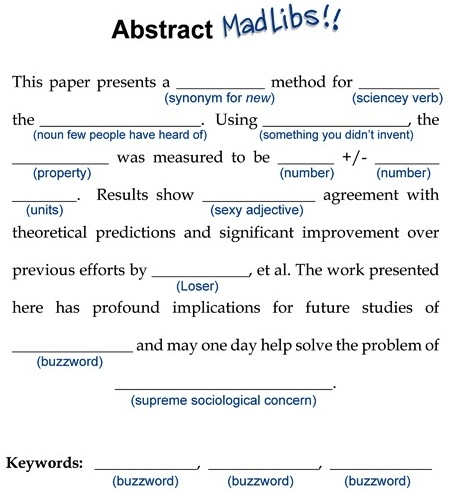
\includegraphics[height=.75\textheight]{phdcomics-abstract.jpg}}
		\end{columns}

	\end{frame}
	
	\subsection{Improving code}
	
	\begin{frame}[t]{Improving \red{code}}

		\textbf{Literate progamming}: \\
		\begin{quote}``Let us change our traditional attitude to the construction of programs: Instead of imagining that our main task is to instruct a computer what to do, let us concentrate rather on\\ \red{explaining to human beings what we want a computer to do}.''\\(Donald Knuth)\end{quote}
			
		\begin{itemize}

			\item \textbf{Variables} should have short and readable names.
			
			\item \textbf{Graphs} should include the \texttt{name()} option to stay in memory.
			
			\item \textbf{Comments} and sections should help understand the code.
		\end{itemize}

		Use the course do-files to find some inspiration and make up your own style of literate programming.
	\end{frame}

	\subsection{Improving graphs}
			
	\begin{frame}[t]{Improving \red{graphs}}

		\begin{itemize}
			
			\item \textbf{Inter-ocular trauma test}: if the graph does not hit you between the eyes, disregard it.

			\begin{itemize}
				\item \texttt{graph box} spots outliers, while \texttt{histogram} qualifies a distribution.
				
				\item \texttt{graph dot} applies to a categorical and a continuous variable.
				\item \texttt{scatter} applies only when the variables are sufficiently continuous.
			\end{itemize}
			
			Save graphs in PNG or PDF format for inclusion into your text.
			
			\item \textbf{Graph options} will make your graphs much more readable and useful: read their documentation, do-files, and ask for help.
			
			\begin{itemize}
				\item \texttt{ylabel(1(10)100)} creates a vertical 100-point labelled scale.
				\item \texttt{yscale(reverse)} reverses the y-axis for a reverse-coded variable.
				\item \texttt{ytitle("GDP growth (\%)")} provides a concise title to the y-axis.
				\item \texttt{mlabel(cname)} adds a label to data points on a scatterplot.
			\end{itemize}
			All graph options are fully documented in Stata. Some options will apply only to the y-axis or x-axis depending on the plot.
		
		\end{itemize}

	\end{frame}

	\subsection{Improving tables}
			
	\begin{frame}[t]{Improving \red{tables}}

		Your do-file produces tons of tables; your final paper shows \red{only two}:
		
		\begin{itemize}
			
			\item \textbf{Descriptive statistics}: \\

			\begin{itemize}
				\item \texttt{sum} or \texttt{tabstat} describe continuous variables.
				\item \texttt{tab} or \texttt{fre} describe categorical variables.
				
				\item \texttt{tabout} export descriptions to text.
			\end{itemize}
			
			\item \textbf{Regression results}: \\
						
			\begin{itemize}
				\item \texttt{reg} and its options produces all regression analysis.
				\item \texttt{mkcorr} exports correlation matrixes to text.
				\item \texttt{estout} exports regression results to text.
			\end{itemize}
		
		\end{itemize}

			Use a spreadsheet editor to import and format your tables, following the options documented in the Stata Guide.\vspace{1em}
			
			Note: presentational aspects are part and parcel of quantitative methods, just like grammar, syntax and punctuation are to writing.
	\end{frame}
	
	\subsection{Systematic proofreading}

	\begin{frame}[t]{Systematic \red{proofreading}}
		\begin{columns}[T]
			\column{.4\textwidth}
			If you forget to proofread your work, a gigantic hole might open in the earth under your feet, and you might burn in the flames of the monstrous Moloc'h for eternity ($p < 0.01$).\vspace{1em}
			
			And your graders will get angry at their laptops.\vspace{1em}
			
			All remaining kittens will be decimated without any sign of human mercifulness.
			\column{.4\textwidth}
			
\includegraphics[height=.66\paperheight]{explain.jpg}
		\end{columns}
	\end{frame}

	\subsection{Further help}
	
	\begin{frame}[t]{Further help}

		\begin{itemize}

			\item Course-specific help:

			\begin{itemize}
				\item Stata Guide
				\item Session do-files
				\item Course slides
			\end{itemize}
	
			\item General help:
			
			\begin{itemize}
				\item Handbook chapters
				\item Stata documentation (\texttt{help \emph{command}})
				\item Online tutorials
			\end{itemize}

		\end{itemize}

		Handbook chapters and course emails are available from the ENTG. Everything else is systematically archived on the course website:\\[.5em]
		
		\url{http://f.briatte.org/teaching/quanti/}\\[.5em]
		
		Happy coding!
		
	\end{frame}
	
	%
	%
	%
	\section{Conclusions}

	\subsection{Concluding thoughts on your data}

	\begin{frame}[t]{Concluding thoughts on your data}
	
	Your Discussion ends the paper by answering some fundamental questions on your research.\\[.5em]
	
	Start with an appraisal of your \red{data}. In the end:\\[.5em]
	
		\begin{itemize}
			\item \textbf{How precise} is your measurement of the issue at stake? Are your variables \red{reliable proxies} for the phenomena you are interested in? What limitations did you run in?
			
			\item \textbf{How representative} is your final sample, on which you ran your model? Would you be able to \red{generalize your results}, to what population and with what confidence?
		\end{itemize}
	
	Data limitations are always expectable in the social sciences. The current data revolution is pushing for open data of higher quality and clarity, but there are serious obstacles and pitfalls.
	
	\end{frame}

	
	\subsection{Concluding thoughts on your model}

	\begin{frame}[t]{Concluding thoughts on your model}
	
	Continue with an appraisal of your \red{model}. In the end:

		\begin{itemize}
			\item \textbf{How predictive} \red{[R-squared]} is your model? Did you manage to formulate a \red{reasonable interpretation} of the relationships that emerged between your variables?
			
			\item \textbf{How informative} was your overall research? Did the interpretation of your model \red{[coefficients]} provide an interesting way to think about your general topic?
		\end{itemize}
	
	By definition, no model perfectly embraces reality. Linear models are extremely sensitive to how you set them up (model specification), and violating their background assumptions is usually devastating.\vspace{1em}
	
	Bayesian statistics are gradually getting us out of this mess.
	
	\end{frame}
					
	\subsection{Concluding thoughts on your methods}

	\begin{frame}[t]{Concluding thoughts on your methods}
	
	Finish with a mental assessment of your \red{methods}:

		\begin{itemize}
			\item \textbf{Our course is introductory}. Much more advanced techniques exist to refine our models.
			
			\item \textbf{Our technique is limited}. Frequentist methods like linear regression have known intrinsic flaws.
			
			\item \textbf{Our knowledge is imperfect}. ``The order of human thought will never reflect the order of things,'' as Simon Shapin puts it.
		\end{itemize}
		
		Further reading:
		
		\begin{itemize}
			\item \textbf{Michel Foucault}, ``The Order of Things'' (1966).
			\item \textbf{Paul Schrodt}, ``Seven Deadly Sins…'' (2010).			 
			\item \textbf{Simon Shapin}, ``Never Pure…'' (2010).
		\end{itemize}
	
	\end{frame}
	
	\section{The end}

	\begin{frame}[t]{Course outline}
	
	\begin{columns}[T]
	\column{.3\textwidth}
	\textbf{Univariate\\statistics}
	
	\vspace{.55em}
	\begin{itemize}
		\item Introduction
		% (analysis of survey data)
		\item Datasets
		% (observations and variables)
		\item Distributions
		% (central tendency, variability, normality)
		\item Estimation
		% (PDF, CLT, LLN, CI, MLE)
	\end{itemize}
	Assignment No. 1
	
	\column{.3\textwidth}
	\textbf{Bivariate\\statistics}
	
	\begin{itemize}
		\item Significance
		% (t-test, comparison of means and proportions)
		\item Crosstabulations
		% (Chi-squared test)
		\item Correlation
		% (scatterplot and correlation matrixes)
		\item Linear regression
		% (Simple OLS linear regression)
	\end{itemize}
	Assignment No. 2
	
	$$
	\left.
    \begin{array}{rrr}
        corrected \\
        revised\\
        appended
    \end{array}
	\right \} 
	$$

	\column{.3\textwidth}
	\textbf{Statistical\\modelling}
	
	\begin{itemize}
		\item Basics
		% (residuals)
		\item Extensions
		% (dummies)
		\item Diagnostics
		% (multicollinearity, heteroscedasticity)
		\item Conclusion
		% (GLS, logistic, ANOVA, Bayesian...)
	\end{itemize}
	\red{Final paper}\\[.5em]
	\fbox{
\includegraphics[width=.75\textwidth]{holy-grail.jpg}}
	\end{columns}
	
	\end{frame}
	
	% ... This is this madness!
	% No...

	\begin{frame}[t,plain]
			\vspace{.3\paperwidth}
		\begin{center}
			
\includegraphics{this-is-stata.jpg}
		\end{center}
	\end{frame}

	\begin{frame}[t,plain]
			\vspace{.3\paperwidth}
		\begin{center}
			{\Large \red{Congratulations}, and thank you.}\\
		\end{center}
			\vspace{1em}
			\hspace{.6\paperwidth}
			\texttt{exit, clear}		
	\end{frame}






	%
	\section{Final paper!}

    %
    %

    \begin{frame}[c]{Thanks for your attention}
    
        \begin{alertblock}{Project}
            \begin{itemize}
                \item Name your paper and do-file like \red{Briatte\_Petev\_2}
                \item Make sure to print your paper to a slick \red{PDF}
            \end{itemize}
        \end{alertblock}
        
        \begin{block}{Readings}
            \begin{itemize}
                \item \emph{Stata Guide}, Sec.~10, 11, 13 and 15
            \end{itemize}
        \end{block}
            
        \begin{exampleblock}{Practice}
            \begin{itemize}
                \item Replicate do-file
                \item \red{Use its structure for Draft No.~2}
            \end{itemize}
        \end{exampleblock}
            
    \end{frame}
    
\end{document}
